\chapter{Futuri sviluppi e integrazioni}
Il progetto qui realizzato rappresenta la base su cui poggerà l'infrastruttura aziendale descritta originariamente nella figura \ref{fig:fsl_general_arch}.
Verranno quindi sostituite le attuali integrazioni con servizi mockup o di terze parti di test con le reali componenti aziendali, ancora in fase di sviluppo internamente.

\section{Threat intelligence}
Il primo punto cruciale con cui si lega a doppio filo è il sistema di Threat Intelligence automatico (di seguito \emph{"T.I."}). Questo, successivamente alla propria ultimazione, si integrerà agli analizzatori statici e dinamici.
Per meglio specificare, lo statico è già predisposto: sarà sufficiente effettuare l'upload sul bucket S3 designato per avviare il processo. Inoltre, per ricevere i risultati, la T.I. esporrà un endpoint HTTP dove ricevere notifiche riguardanti l'avvio, la terminazione o eventuali errori di un task relativo a un sample caricato.
Questo sistema di notifiche segue il paradigma dei webhook, ossia un sistema di callback implementato a livello di richieste HTTP. In questo modo, già predisposto, il richiedente non dovrà attendere anche svariati minuti con la connessione TCP aperta finché il server non abbia terminato la propria elaborazione, con il rischio di perdere tutto in caso di interruzioni di rete. Al contrario, gestirà l'avanzamento tramite endpoint dedicati, senza dover allocare risorse durante l'esecuzione.
Questa integrazione è resa dal progetto estremamente facile, perché le librerie per eseguire richieste HTTP sono già incluse, assieme alla definizione dei tipi di dati scambiati.
Siccome questa modifica sarà obbligata, nel codice sono stati inseriti dei commenti \emph{TODO} esattamente nei punti specifici dove cambiare tale comportamento, al fine di rendere la loro identificazione molto semplice per lo sviluppatore che lavorerà con questo progetto in futuro.

Un sistema più avanzato potrebbe prevedere l'uso di code FIFO per i messaggi. AWS implementa tale funzionalità attraverso il proprio prodotto denominato \textbf{SQS} (\emph{Simple Queue Service}), dove l'analizzatore avrà il ruolo di producer e il richiedente sarà il consumer. Così si aumenta la \emph{fault tolerance}, essendo che i messaggi di output resteranno nella coda, lasciando tutto il tempo al servizio della T.I. di tornare in funzione, senza perdere dati.

\begin{figure}[htbp]
    \centering
    \begin{subfigure}[t]{0.48\textwidth}
        \centering
        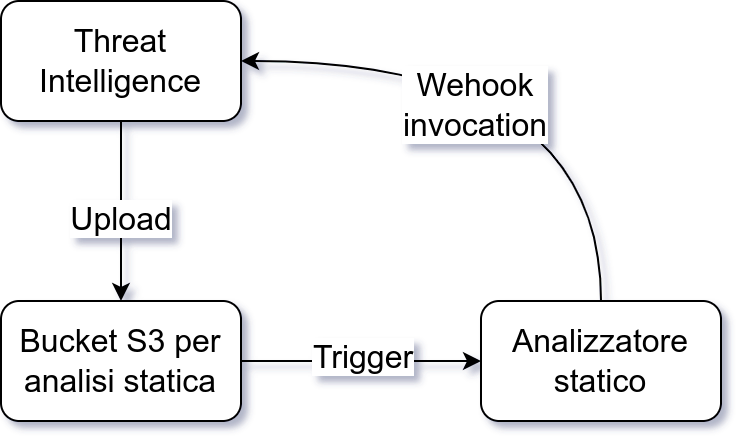
\includegraphics[width=\textwidth]{assets/ti_webhook.png}
        \caption{Risposta mediante webhook}
    \end{subfigure}
    \begin{subfigure}[t]{0.48\textwidth}
        \centering
        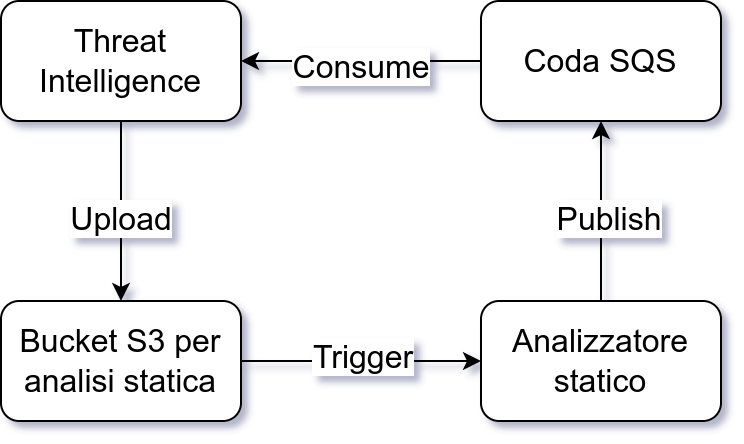
\includegraphics[width=\textwidth]{assets/ti_sqs.png}
        \caption{Risposta mediante uso di coda SQS}
    \end{subfigure}
    \caption{Potenziali integrazioni tra la T.I. e l'analizzatore statico}
    \label{fig:future_threat_intell_analyzer_integrations}
\end{figure}

\bigskip

Passando a integrare anche l'analizzatore dinamico, ciò comporterebbe il piccolo sviluppo di una API, possibilmente REST, che consenta di invocare l'analisi per dei sample specifici.
Come accennato in precedenza, non deve essere eseguito un task in concomitanza alla parte statica. Questo perchè deve essere compito della Threat Intelligence, o dell'analista in persona, decidere se ha senso spendere risorse nell'analisi dinamica o meno, sulla base dei risultati della prima o l'uso di una threshold di confidence determinata secondo i più svariati criteri.

La soluzione per cui il progetto è stato predisposto è la seguente:
\begin{itemize}
    \item Viene realizzata una REST API, che espone un endpoint per l'avvio di un task di analisi dato il sample, e che dialoga con Cuckoo utilizzando come base il modulo Python costruito nella sezione \ref{sez:dynamic-python-client-vm}: per via della libreria già pronta e testata, lo sforzo umano richiesto si prevede sia notevolmente basso
    \item La T.I. andrà ad esporre un suo webhook per la ricezione della risposta o degli errori provenienti dalla Sandbox
    \item La VM con l'analizzatore, al termine del task, dove ora semplicemente salva i risultati negli appositi file e mostra l'output di successo all'utente, andrà a invocare il webhook di callback inviando i risultati; in alternativa potrebbero essere caricati su un bucket S3 a fini di archiviazione
\end{itemize}

\begin{figure}[htbp]
    \centering
    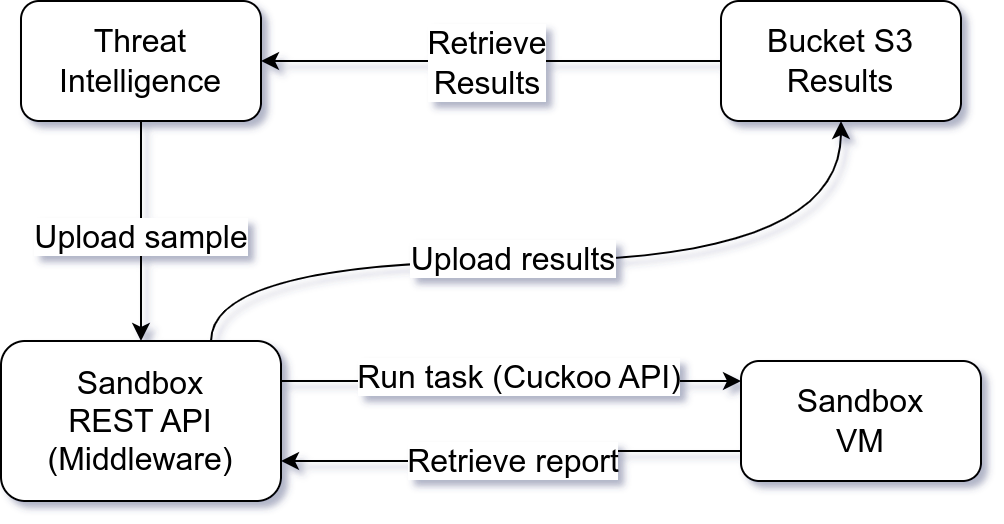
\includegraphics[width=0.7\textwidth]{assets/future_dynamic_ti_integration.png}
    \caption{Possibile integrazione futura della sandbox con la Threat Intelligence}
    \label{fig:future_dynamic_ti_integration}
\end{figure}

Com'è possibile notare, si tratta di operazioni relativamente semplici, che non richiedono un grande quantitativo di forza lavoro.
Questo è il risultato positivo derivante dall'architettura del progetto, mantenendo il focus sempre sulla scalabilità e adattabilità dello strumento.
Tuttavia, la parte più dispendiosa, potrebbe riguardare l'acquisto e l'impostazione iniziale di un server fisico reale predisposto per l'esecuzione della sandbox.

\section{VPN}
Un fattore che potrebbe permettere al malware di capire che si trova sotto analisi da parte di un'azienda di sicurezza, è l'indirizzo IP pubblico col quale dialoga su Internet.
Nel caso di un agent C\&C (command and control), il malintenzionato vedrebbe comparire nel proprio pool di computer infettati anche una connessione avente per capo un IP pubblico. Potrebbe andare ad eseguire un reverse DNS su tale indirizzo, scoprendo facilmente che appartiene a un'azienda di cybersecurity.
L'effetto finale è quello che l'attaccante non andrà presumibilmente a far eseguire a quel computer (di fatto la nostra VM con Windows 7) payload malevoli, ma bensì potrebbe ordinare l'autodistruzione e andare ad applicare strategie di mitigazione, come il cambio dell'host centro di comando.

Una soluzione efficace è quella di inserire la sandbox all'interno di una VPN retail, aiutata dal loro sempre maggiore utilizzo da parte degli utenti comuni. Così facendo, le richieste verso Internet verrebbero viste dall'attaccante come provenienti da un servizio VPN usato da milioni di utenti per il mondo, nascondendo il fatto che si tratti di un'azienda specializzata nel settore.

\begin{figure}[htbp]
    \centering
    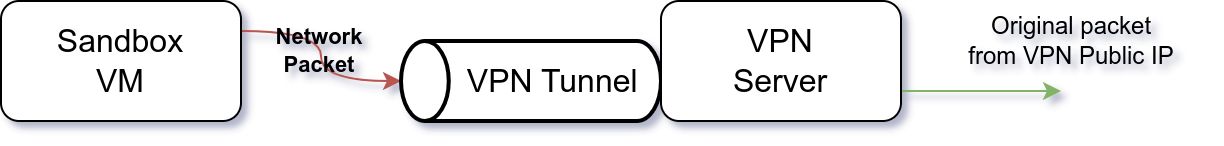
\includegraphics[width=\textwidth]{assets/sandbox_vpn.png}
    \caption{Transito dei pacchetti di rete dalla sandbox alla VPN verso Internet}
    \label{fig:sandbox_vpn_diagram}
\end{figure}

\section{Deploy totale su AWS}
Un passaggio che si è valutato durante l'esecuzione del progetto è stato quello di far eseguire le macchine virtuali direttamente su cloud attraverso servizi AWS, al posto di adoperare un server fisico aziendale.
Ciò minimizzerebbe i rischi di evasion e infezione del resto dell'infrastruttura aziendale locale, ma non va dimenticato l'aspetto relativo alla fattibilità tecnica e legale. Bisogna tenere conto che è richiesto che l'host fisico su cui esegue la sandbox supporti sia la virtualizzazione standard che innestata. Quest'ultima non è molto comune tra i server AWS poiché non se ne vedono applicazioni più generiche. Infine, sarà una migrazione valutabile solo a posteriori di una consulenza legale per assicurarsi di non violare i termini di utilizzo di AWS, nello specifico dei prodotti di EC2 (per il server), nonché dell'infrastruttura di rete su cui transiterebbe indisturbato del traffico potenzialmente malevolo o facente parte di una botnet.

\section{Uso di Cuckoo Sandbox su Python 3}
È stato sottolineato come sia stato utilizzato il software Cuckoo Sandbox nella versione originale, realizzata dalla Cuckoo Foundation, scritta in Python 2. Oltre a dipendere da una versione dell'interprete ormai deprecata e da librerie obsolete, sia perché non più mantenute che non più riceventi aggiornamenti di sicurezza, anche il progetto stesso è stato archiviato e non vedrà migliorie future, come chiaramente esplicitato sulla propria pagina GitHub.
\footnote{Annunciato nel README al link \url{https://github.com/cuckoosandbox/cuckoo/commit/50452a39ff7c3e0c4c94d114bc6317101633b958}}

Tutto ciò è dovuto dalla riscrittura della nuova versione basata su Python 3, che inevitabilmente romperà la retrocompatibilità con l'attuale.
Non è stata usata in questo progetto perché ancora non disponibile al pubblico, ma è programmato il suo utilizzo in una fase futura, dopo che sarà dichiarata stabile e testata a sufficienza. Inoltre, per l'uso per il quale verrà sfruttata, l'azienda richiederà che vengano prima effettuati approfonditi security audit, per verificare che non presenti evidenti vulnerabilità di sicurezza che potrebbero compromettere il sistema per intero.
